\documentclass[12pt]{paper}
\RequirePackage{filecontents}
\begin{filecontents}{pp.bib}
	@protocol{
		openid,
		title = {{OpenId Connect}},
		year = {2007},
		author = {{Fitzpatrick, Brad}},
		note = {\url{https://openid.net/}}
	},
	@online{todoist,
		author = {{Doist}},
		title = {{Todoist}},
		note = {\url{https://todoist.com/}}
	},
	@article{
		neural-net,
		title = {{Neural Networks}},
		author = {{Gurney, Kevin}},
		year = {1997},
		note = {\url{http://www.macs.hw.ac.uk/~yjc32/project/ref-NN/Gurney_et_al.pdf}}
	},
	@online{google-calendar,
		title = {Google Calendar},
		url = {https://calendar.google.com/},
		OPTorganization = {Google},
	},
	@online{dataset,
		title = {The IAM-database: An English Sentence Database for Off-line Handwriting Recognition},
		note = {\url{https://fki.tic.heia-fr.ch/databases/iam-handwriting-database}},
		author = {{U. Marti, H. Bunke}}
	},
	@online{rest,
		title = {REST},
		note = {\url{https://www.ics.uci.edu/~fielding/pubs/dissertation/rest_arch_style.htm}},
		author = {{Fielding, Roy Thomas}},
		year = {2000}
	}
	
\end{filecontents}
\usepackage{graphicx}
\usepackage{hyperref}
\usepackage[english]{babel}
\usepackage{setspace}
\usepackage{indentfirst}
\usepackage[utf8]{inputenc}
\usepackage{fancyhdr}
\usepackage{tabu}
\usepackage{setspace}
\pagestyle{plain}
\fancyhf{} % sets both header and footer to nothing
\renewcommand{\headrulewidth}{0pt}
\usepackage[document]{ragged2e}
\pagenumbering{arabic}
\renewcommand{\labelenumii}{\theenumii}
\renewcommand{\theenumii}{\theenumi.\arabic{enumii}.}
\usepackage[hmargin=1.5cm,vmargin=1.5cm,bmargin=1.5cm]{geometry}
\title{
	\vspace{-50mm}
	\begin{minipage}[l]{\textwidth}
		\hspace{-20mm}\resizebox{75mm}{!}{
\includegraphics{./images/logoISEL.png}}
	\end{minipage}
}

\author{
	\begin{tabular}{ll}
		& Bernardo Rodrigues\\[50mm]
	\end{tabular}
}

\date{
	\begin{tabular}{ll}
		{Supervisors: }&& Nuno Leite\\
	\end{tabular}[10mm]
}



\begin{document}
		\begin{figure}[!ht]
			\centering
			\hspace{-20mm}\resizebox{75mm}{!}{
\includegraphics{./images/logoISEL.png}}\\
%			\scalebox{0.6}{\includegraphics{images/Logo_ISEL}}
		\end{figure}	
		
		\begin{center}
			{\huge ToDo - System for managing user's To Do list}\\
			\vspace{1cm}
			{\Large Engenharia Informática e Computadores}\\
			{\large Projecto e Seminário - 2020/21}
		\end{center}
	
		\vspace{1cm}
		
		\begin{itemize}
			\item[] Bernardo Rodrigues, n. 42130
			\\ \href{mailto:A42130@alunos.isel.pt}{A42130@alunos.isel.pt}
		\end{itemize}
		\vspace{1cm}
		\begin{center}
			\centering
			Supervisor:
			\\
			Nuno Leite, ISEL, \href{mailto:nuno.leite@isel.pt}{nuno.leite@isel.pt}
		\end{center}
		
		\rfoot{\today}
	\vspace{1cm}
	
	\section{Introduction}
		\setlength{\parindent}{0.5cm}
		In today's fast and complex world people try to schedule days or weeks. We create small reminders, either virtually or physically, to do something, whatever that may be. Those little notes we give to ourselves, those "to-do's" are often forgotten and not fully fulfilled. As such this application will attempt to mend that by creating an environment where a reminder is easily created but hardly forgotten or skipped over.
		This application will allow the users to create an account and then create reminders by either writing them or taking a picture of a post-it.
	
	\section{State of the Art}
		\setlength{\parindent}{0.5cm}
		The need to organize our daily lives isn't a new concept and as such, to-do applications are not new. A few examples of some of these are \textit{Todoist \cite{todoist}}, and Google Calendar's reminder system \cite{google-calendar}.
		The main difference between these applications and the one being developed in this project is the image recognition component as well as the prioritization algorithm.
	
	

	\section{Proposed Solution}
		\setlength{\parindent}{0.5cm}
		The goal of the project is to create a web application using current practices and technologies. The application will be comprised of a web \textit{API}, a database and front-end application as shown below.\\
		\begin{figure}[!h]
			\centering
			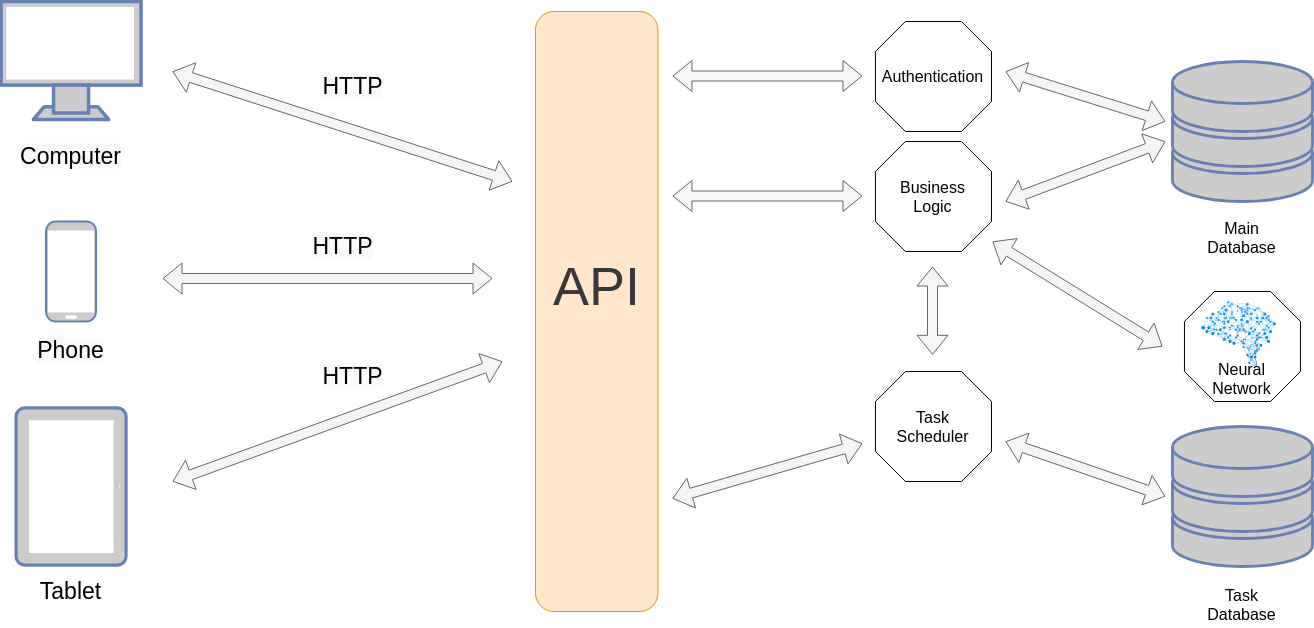
\includegraphics[width=150mm,scale=0.8]{./images/abstract-architecture-Page-2.png}
			\caption{Abstract architecture of the solution}
		\end{figure}
%		\vspace{0.5cm}
		
		The proposed solution is intended to be generic and expandable for future use.
		The user will be able to create, delete and edit new reminders or "to-do's" and assign them a priority as well as a date. The application will then rank these to-do's and arrange them in a way where the user will not forget them and will actually fulfill them. This will be achieved using a \textit{REST \cite{rest}} \textit{API} with a push notifications component.
		
		There will be a ranking algorithm designed to prioritize these ``to-do's`` and then remind the user to fulfill them.
		This \textit{API} will have an image recognition component that will recognize writing on post-it's for a better user experience.
		
		The image recognition component will be achieved by creating, modeling and training a neural network\cite{neural-net}. The training will be achieved using a \textit{dataset \cite{dataset}} with 657 different writers.

	\setcounter{page}{2}
	\section{Required Functionalities}
		\begin{enumerate}
			\item Allow users to sign up, log in, log out and delete the account.
			\item Create, edit and erase to-do's.
			\item To-do's ranking algorithm.
			\begin{enumerate}
				\item Rank to-do's based on date and priority
				\item Push notifications.
			\end{enumerate}
			\item Image recognition creation based on post-it's (English only).
		\end{enumerate}
	
	\section{Optional Functionalities}
		\begin{enumerate}
			\item \textit{OpenId \cite{openid}} log in.
			\item Profile Picture.
		\end{enumerate}
	\section{Schedule}
	\begin{figure}[h]
		\centering
		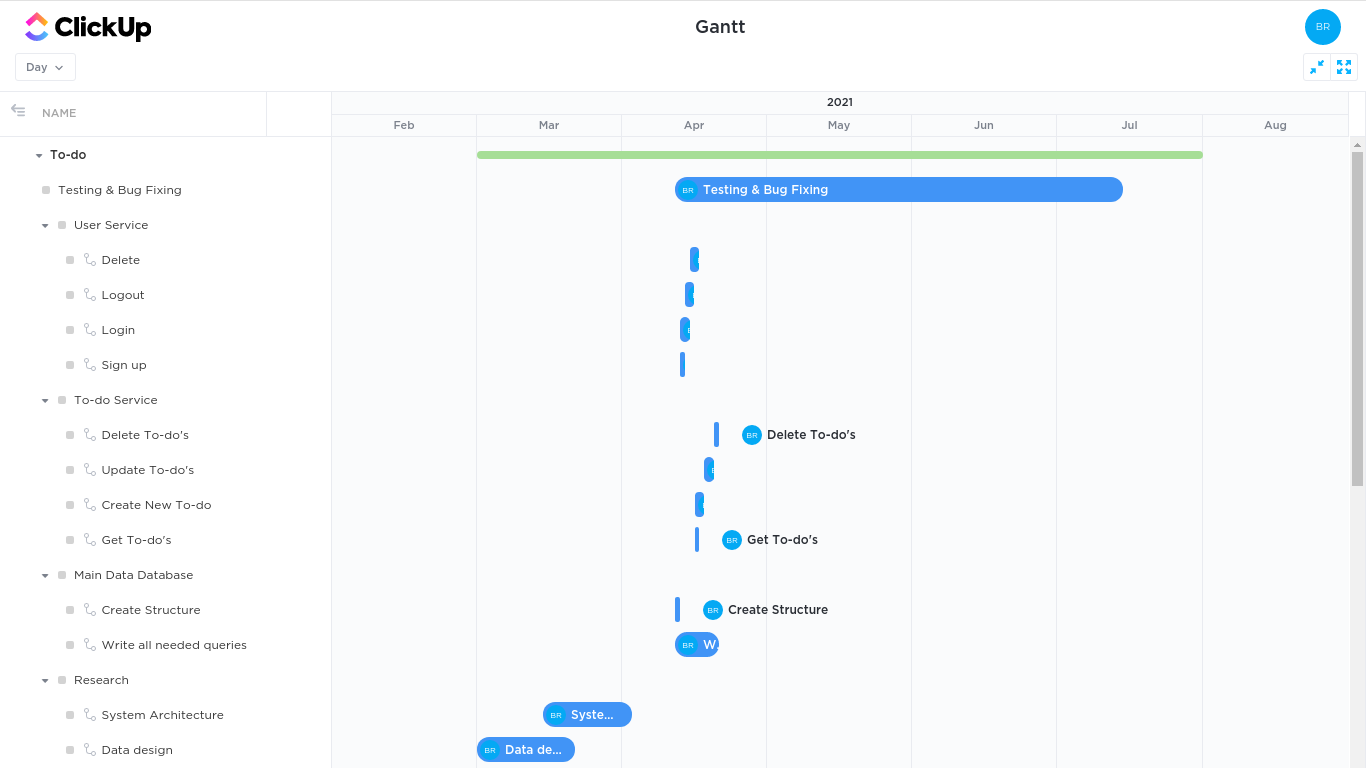
\includegraphics[width=150mm,scale=0.5]{./images/gantt-chart-1.png}
	\end{figure}
	\begin{figure}[!h]
		\centering
		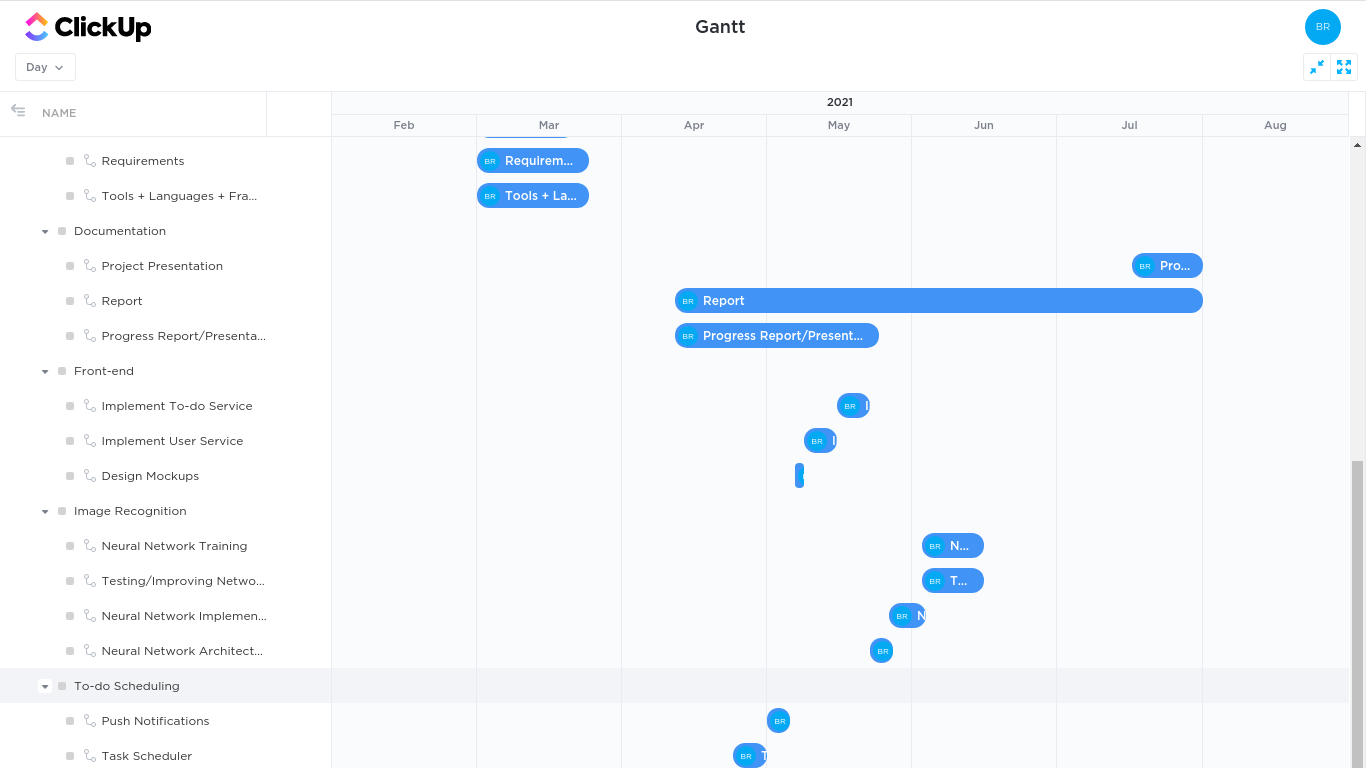
\includegraphics[width=150mm,scale=0.5]{./images/gantt-chart-2.png}
		\caption{Gantt chart}
	\end{figure}
	\href{https://share.clickup.com/g/h/4g659-29/c4e331e430e363e}{For a better look at the Gantt chart}
	\pagebreak
	\bibliographystyle{plain}
	\bibliography{pp}


\end{document}